% Schema
\section{Userspace}
	\begin{frame}
		\begin{figure}
		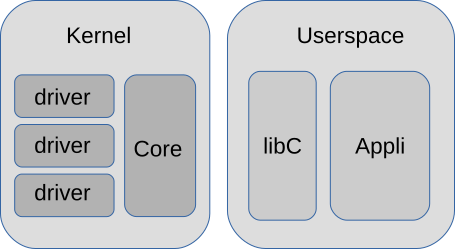
\includegraphics[height=4cm]{img/arch_linux_full.png}
		\caption{kernel + userspace}
		\end{figure}
	\end{frame}
	\begin{frame}
		\center{\huge{Système d'init}}
		\begin{itemize}
			\item Premier processus lancé
			\item Lance les autres processus
			\item Influe sur le temps de boot
		\end{itemize}
		\begin{block}{SysV init}
			\begin{itemize}
				\item Scripts
				\item Peu de parallélisation
			\end{itemize}
		\end{block}
		\begin{block}{Systemd}
			\begin{itemize}
				\item Fichiers de configuration
				\item Parallélisation et dépendances
				\item Plus complexe
			\end{itemize}
		\end{block}
	\end{frame}

	\begin{frame}
		\begin{block}{Librairies}
			\begin{itemize}
				\item libC : GNU libC, uClibC, dietlibC
				\item librairies métier
			\end{itemize}
		\end{block}
		\begin{block}{Utilitaires}
			\begin{itemize}
				\item Commandes standard : GNU Coreutils, Busybox
				\item Applications métier
				\item Daemons système
			\end{itemize}
		\end{block}
	Choix dicté par les contraintes de stockage.
	\end{frame}

